\mbox{$\displaystyle +\,\frac{1}{4}$\,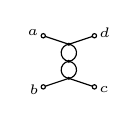
\begin{tikzpicture}[x=0.340cm, y=0.340cm, line width=0.420pt, baseline={([yshift=-0.6ex]0,0)}]
  \draw (-0.955,0.955) -- (0.000,0.636);
  \draw (-0.955,-0.955) -- (0.000,-0.636);
  \draw (0.955,-0.955) -- (0.000,-0.636);
  \draw (0.955,0.955) -- (0.000,0.636);
  \draw (0.000,0.000) arc[start angle=276.026, end angle=443.974, radius=0.320];
  \draw (0.000,0.000) arc[start angle=263.974, end angle=96.026, radius=0.320];
  \draw (0.000,0.000) arc[start angle=96.026, end angle=263.974, radius=0.320];
  \draw (0.000,0.000) arc[start angle=83.974, end angle=-83.974, radius=0.320];
  \fill (0.000,0.000) circle (0.064);
  \fill (0.000,0.636) circle (0.064);
  \fill (0.000,-0.636) circle (0.064);
  \draw[fill=white] (-0.955,0.955) circle (0.080);
  \draw[fill=white] (-0.955,-0.955) circle (0.080);
  \draw[fill=white] (0.955,-0.955) circle (0.080);
  \draw[fill=white] (0.955,0.955) circle (0.080);
  \node[font=\tiny, inner sep=0pt, anchor=342] at (-1.116,1.008) {$a$};
  \node[font=\tiny, inner sep=0pt, anchor=18] at (-1.116,-1.008) {$b$};
  \node[font=\tiny, inner sep=0pt, anchor=162] at (1.116,-1.008) {$c$};
  \node[font=\tiny, inner sep=0pt, anchor=198] at (1.116,1.008) {$d$};
\end{tikzpicture}}
\diagramgap
\mbox{$\displaystyle +\,\frac{1}{4}$\,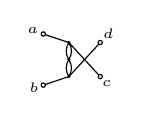
\begin{tikzpicture}[x=0.340cm, y=0.340cm, line width=0.420pt, baseline={([yshift=-0.6ex]0,0)}]
  \draw (-0.955,0.955) -- (0.000,0.636);
  \draw (-0.955,-0.955) -- (0.000,-0.636);
  \draw (1.173,-0.636) -- (0.000,0.636);
  \draw (1.173,0.636) -- (0.000,-0.636);
  \draw (0.000,0.000) arc[start angle=325.937, end angle=394.063, radius=0.568];
  \draw (0.000,0.000) arc[start angle=214.063, end angle=145.937, radius=0.568];
  \draw (0.000,0.000) arc[start angle=145.937, end angle=214.063, radius=0.568];
  \draw (0.000,0.000) arc[start angle=34.063, end angle=-34.063, radius=0.568];
  \fill (0.000,0.000) circle (0.064);
  \fill (0.000,0.636) circle (0.064);
  \fill (0.000,-0.636) circle (0.064);
  \draw[fill=white] (-0.955,0.955) circle (0.080);
  \draw[fill=white] (-0.955,-0.955) circle (0.080);
  \draw[fill=white] (1.173,-0.636) circle (0.080);
  \draw[fill=white] (1.173,0.636) circle (0.080);
  \node[font=\tiny, inner sep=0pt, anchor=342] at (-1.116,1.008) {$a$};
  \node[font=\tiny, inner sep=0pt, anchor=18] at (-1.116,-1.008) {$b$};
  \node[font=\tiny, inner sep=0pt, anchor=133] at (1.288,-0.761) {$c$};
  \node[font=\tiny, inner sep=0pt, anchor=227] at (1.288,0.761) {$d$};
\end{tikzpicture}}
\diagramgap
\mbox{$\displaystyle +\,\frac{1}{4}$\,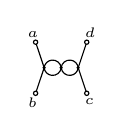
\begin{tikzpicture}[x=0.340cm, y=0.340cm, line width=0.420pt, baseline={([yshift=-0.6ex]0,0)}]
  \draw (-0.955,0.955) -- (-0.636,0.000);
  \draw (-0.955,-0.955) -- (-0.636,0.000);
  \draw (0.955,-0.955) -- (0.636,0.000);
  \draw (0.955,0.955) -- (0.636,0.000);
  \draw (0.000,0.000) arc[start angle=6.026, end angle=173.974, radius=0.320];
  \draw (0.000,0.000) arc[start angle=353.974, end angle=186.026, radius=0.320];
  \draw (0.000,0.000) arc[start angle=186.026, end angle=353.974, radius=0.320];
  \draw (0.000,0.000) arc[start angle=173.974, end angle=6.026, radius=0.320];
  \fill (0.000,0.000) circle (0.064);
  \fill (-0.636,0.000) circle (0.064);
  \fill (0.636,0.000) circle (0.064);
  \draw[fill=white] (-0.955,0.955) circle (0.080);
  \draw[fill=white] (-0.955,-0.955) circle (0.080);
  \draw[fill=white] (0.955,-0.955) circle (0.080);
  \draw[fill=white] (0.955,0.955) circle (0.080);
  \node[font=\tiny, inner sep=0pt, anchor=288] at (-1.008,1.116) {$a$};
  \node[font=\tiny, inner sep=0pt, anchor=72] at (-1.008,-1.116) {$b$};
  \node[font=\tiny, inner sep=0pt, anchor=108] at (1.008,-1.116) {$c$};
  \node[font=\tiny, inner sep=0pt, anchor=252] at (1.008,1.116) {$d$};
\end{tikzpicture}}
\diagramgap
\mbox{$\displaystyle +\,\frac{1}{4}$\,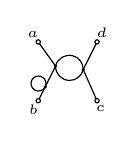
\begin{tikzpicture}[x=0.340cm, y=0.340cm, line width=0.420pt, baseline={([yshift=-0.6ex]0,0)}]
  \draw (-1.098,1.098) -- (-0.452,0.194);
  \draw (-1.098,-1.098) -- (-0.839,-0.581);
  \draw (1.098,-1.098) -- (0.581,0.065);
  \draw (1.098,1.098) -- (0.581,0.065);
  \draw (-0.452,0.194) -- (-0.839,-0.581);
  \draw (-0.452,0.194) arc[start angle=178.901, end angle=346.849, radius=0.524];
  \draw (-0.452,0.194) arc[start angle=166.849, end angle=-1.099, radius=0.524];
  \draw (-0.839,-0.581) arc[start angle=333.435, end angle=693.435, radius=0.280];
  \fill (-0.452,0.194) circle (0.064);
  \fill (-0.839,-0.581) circle (0.064);
  \fill (0.581,0.065) circle (0.064);
  \draw[fill=white] (-1.098,1.098) circle (0.080);
  \draw[fill=white] (-1.098,-1.098) circle (0.080);
  \draw[fill=white] (1.098,-1.098) circle (0.080);
  \draw[fill=white] (1.098,1.098) circle (0.080);
  \node[font=\tiny, inner sep=0pt, anchor=306] at (-1.197,1.236) {$a$};
  \node[font=\tiny, inner sep=0pt, anchor=63] at (-1.174,-1.250) {$b$};
  \node[font=\tiny, inner sep=0pt, anchor=114] at (1.167,-1.253) {$c$};
  \node[font=\tiny, inner sep=0pt, anchor=243] at (1.174,1.250) {$d$};
\end{tikzpicture}}
\diagramgap
\mbox{$\displaystyle +\,\frac{1}{4}$\,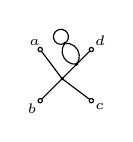
\begin{tikzpicture}[x=0.340cm, y=0.340cm, line width=0.420pt, baseline={([yshift=-0.6ex]0,0)}]
  \draw (-0.955,0.955) -- (-0.136,-0.136);
  \draw (-0.955,-0.955) -- (-0.136,-0.136);
  \draw (0.955,-0.955) -- (-0.136,-0.136);
  \draw (0.955,0.955) -- (0.409,0.409);
  \draw (-0.042,1.188) arc[start angle=143.594, end angle=276.612, radius=0.491];
  \draw (-0.042,1.188) arc[start angle=96.612, end angle=-36.406, radius=0.491];
  \draw (0.409,0.409) -- (-0.136,-0.136);
  \draw (-0.042,1.188) arc[start angle=300.103, end angle=660.103, radius=0.280];
  \fill (-0.042,1.188) circle (0.064);
  \fill (0.409,0.409) circle (0.064);
  \fill (-0.136,-0.136) circle (0.064);
  \draw[fill=white] (-0.955,0.955) circle (0.080);
  \draw[fill=white] (-0.955,-0.955) circle (0.080);
  \draw[fill=white] (0.955,-0.955) circle (0.080);
  \draw[fill=white] (0.955,0.955) circle (0.080);
  \node[font=\tiny, inner sep=0pt, anchor=307] at (-1.057,1.091) {$a$};
  \node[font=\tiny, inner sep=0pt, anchor=45] at (-1.075,-1.075) {$b$};
  \node[font=\tiny, inner sep=0pt, anchor=143] at (1.091,-1.057) {$c$};
  \node[font=\tiny, inner sep=0pt, anchor=225] at (1.075,1.075) {$d$};
\end{tikzpicture}}
\diagramgap
\mbox{$\displaystyle +\,\frac{1}{4}$\,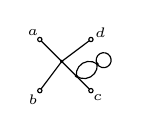
\begin{tikzpicture}[x=0.340cm, y=0.340cm, line width=0.420pt, baseline={([yshift=-0.6ex]0,0)}]
  \draw (-0.955,0.955) -- (-0.136,0.136);
  \draw (-0.955,-0.955) -- (-0.136,0.136);
  \draw (0.955,-0.955) -- (0.409,-0.409);
  \draw (0.955,0.955) -- (-0.136,0.136);
  \draw (1.188,0.042) arc[start angle=53.594, end angle=186.612, radius=0.491];
  \draw (1.188,0.042) arc[start angle=6.612, end angle=-126.406, radius=0.491];
  \draw (0.409,-0.409) -- (-0.136,0.136);
  \draw (1.188,0.042) arc[start angle=210.103, end angle=570.103, radius=0.280];
  \fill (1.188,0.042) circle (0.064);
  \fill (0.409,-0.409) circle (0.064);
  \fill (-0.136,0.136) circle (0.064);
  \draw[fill=white] (-0.955,0.955) circle (0.080);
  \draw[fill=white] (-0.955,-0.955) circle (0.080);
  \draw[fill=white] (0.955,-0.955) circle (0.080);
  \draw[fill=white] (0.955,0.955) circle (0.080);
  \node[font=\tiny, inner sep=0pt, anchor=315] at (-1.075,1.075) {$a$};
  \node[font=\tiny, inner sep=0pt, anchor=53] at (-1.057,-1.091) {$b$};
  \node[font=\tiny, inner sep=0pt, anchor=135] at (1.075,-1.075) {$c$};
  \node[font=\tiny, inner sep=0pt, anchor=217] at (1.091,1.057) {$d$};
\end{tikzpicture}}
\diagramgap
\mbox{$\displaystyle +\,\frac{1}{4}$\,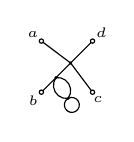
\begin{tikzpicture}[x=0.340cm, y=0.340cm, line width=0.420pt, baseline={([yshift=-0.6ex]0,0)}]
  \draw (-0.955,0.955) -- (0.136,0.136);
  \draw (-0.955,-0.955) -- (-0.409,-0.409);
  \draw (0.955,-0.955) -- (0.136,0.136);
  \draw (0.955,0.955) -- (0.136,0.136);
  \draw (0.042,-1.188) arc[start angle=323.594, end angle=456.612, radius=0.491];
  \draw (0.042,-1.188) arc[start angle=276.612, end angle=143.594, radius=0.491];
  \draw (-0.409,-0.409) -- (0.136,0.136);
  \draw (0.042,-1.188) arc[start angle=120.103, end angle=480.103, radius=0.280];
  \fill (0.042,-1.188) circle (0.064);
  \fill (-0.409,-0.409) circle (0.064);
  \fill (0.136,0.136) circle (0.064);
  \draw[fill=white] (-0.955,0.955) circle (0.080);
  \draw[fill=white] (-0.955,-0.955) circle (0.080);
  \draw[fill=white] (0.955,-0.955) circle (0.080);
  \draw[fill=white] (0.955,0.955) circle (0.080);
  \node[font=\tiny, inner sep=0pt, anchor=323] at (-1.091,1.057) {$a$};
  \node[font=\tiny, inner sep=0pt, anchor=45] at (-1.075,-1.075) {$b$};
  \node[font=\tiny, inner sep=0pt, anchor=127] at (1.057,-1.091) {$c$};
  \node[font=\tiny, inner sep=0pt, anchor=225] at (1.075,1.075) {$d$};
\end{tikzpicture}}
\diagramgap
\mbox{$\displaystyle +\,\frac{1}{4}$\,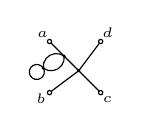
\begin{tikzpicture}[x=0.340cm, y=0.340cm, line width=0.420pt, baseline={([yshift=-0.6ex]0,0)}]
  \draw (-0.955,0.955) -- (-0.409,0.409);
  \draw (-0.955,-0.955) -- (0.136,-0.136);
  \draw (0.955,-0.955) -- (0.136,-0.136);
  \draw (0.955,0.955) -- (0.136,-0.136);
  \draw (-1.188,-0.042) arc[start angle=233.594, end angle=366.612, radius=0.491];
  \draw (-1.188,-0.042) arc[start angle=186.612, end angle=53.594, radius=0.491];
  \draw (-0.409,0.409) -- (0.136,-0.136);
  \draw (-1.188,-0.042) arc[start angle=30.103, end angle=390.103, radius=0.280];
  \fill (-1.188,-0.042) circle (0.064);
  \fill (-0.409,0.409) circle (0.064);
  \fill (0.136,-0.136) circle (0.064);
  \draw[fill=white] (-0.955,0.955) circle (0.080);
  \draw[fill=white] (-0.955,-0.955) circle (0.080);
  \draw[fill=white] (0.955,-0.955) circle (0.080);
  \draw[fill=white] (0.955,0.955) circle (0.080);
  \node[font=\tiny, inner sep=0pt, anchor=315] at (-1.075,1.075) {$a$};
  \node[font=\tiny, inner sep=0pt, anchor=37] at (-1.091,-1.057) {$b$};
  \node[font=\tiny, inner sep=0pt, anchor=135] at (1.075,-1.075) {$c$};
  \node[font=\tiny, inner sep=0pt, anchor=233] at (1.057,1.091) {$d$};
\end{tikzpicture}}
\diagramgap
\mbox{$\displaystyle +\,\frac{1}{6}$\,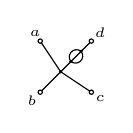
\begin{tikzpicture}[x=0.340cm, y=0.340cm, line width=0.420pt, baseline={([yshift=-0.6ex]0,0)}]
  \draw (-0.955,0.955) -- (-0.191,-0.191);
  \draw (-0.955,-0.955) -- (-0.191,-0.191);
  \draw (0.955,-0.955) -- (-0.191,-0.191);
  \draw (0.955,0.955) -- (0.573,0.573);
  \draw (0.573,0.573) arc[start angle=51.026, end angle=218.974, radius=0.271];
  \draw (0.573,0.573) -- (0.191,0.191);
  \draw (0.573,0.573) arc[start angle=38.974, end angle=-128.974, radius=0.271];
  \draw (0.191,0.191) -- (-0.191,-0.191);
  \fill (0.573,0.573) circle (0.064);
  \fill (0.191,0.191) circle (0.064);
  \fill (-0.191,-0.191) circle (0.064);
  \draw[fill=white] (-0.955,0.955) circle (0.080);
  \draw[fill=white] (-0.955,-0.955) circle (0.080);
  \draw[fill=white] (0.955,-0.955) circle (0.080);
  \draw[fill=white] (0.955,0.955) circle (0.080);
  \node[font=\tiny, inner sep=0pt, anchor=304] at (-1.049,1.096) {$a$};
  \node[font=\tiny, inner sep=0pt, anchor=45] at (-1.075,-1.075) {$b$};
  \node[font=\tiny, inner sep=0pt, anchor=146] at (1.096,-1.049) {$c$};
  \node[font=\tiny, inner sep=0pt, anchor=225] at (1.075,1.075) {$d$};
\end{tikzpicture}}
\diagramgap
\mbox{$\displaystyle +\,\frac{1}{6}$\,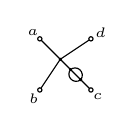
\begin{tikzpicture}[x=0.340cm, y=0.340cm, line width=0.420pt, baseline={([yshift=-0.6ex]0,0)}]
  \draw (-0.955,0.955) -- (-0.191,0.191);
  \draw (-0.955,-0.955) -- (-0.191,0.191);
  \draw (0.955,-0.955) -- (0.573,-0.573);
  \draw (0.955,0.955) -- (-0.191,0.191);
  \draw (0.573,-0.573) arc[start angle=321.026, end angle=488.974, radius=0.271];
  \draw (0.573,-0.573) -- (0.191,-0.191);
  \draw (0.573,-0.573) arc[start angle=308.974, end angle=141.026, radius=0.271];
  \draw (0.191,-0.191) -- (-0.191,0.191);
  \fill (0.573,-0.573) circle (0.064);
  \fill (0.191,-0.191) circle (0.064);
  \fill (-0.191,0.191) circle (0.064);
  \draw[fill=white] (-0.955,0.955) circle (0.080);
  \draw[fill=white] (-0.955,-0.955) circle (0.080);
  \draw[fill=white] (0.955,-0.955) circle (0.080);
  \draw[fill=white] (0.955,0.955) circle (0.080);
  \node[font=\tiny, inner sep=0pt, anchor=315] at (-1.075,1.075) {$a$};
  \node[font=\tiny, inner sep=0pt, anchor=56] at (-1.049,-1.096) {$b$};
  \node[font=\tiny, inner sep=0pt, anchor=135] at (1.075,-1.075) {$c$};
  \node[font=\tiny, inner sep=0pt, anchor=214] at (1.096,1.049) {$d$};
\end{tikzpicture}}
\diagramgap
\mbox{$\displaystyle +\,\frac{1}{6}$\,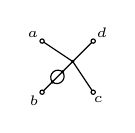
\begin{tikzpicture}[x=0.340cm, y=0.340cm, line width=0.420pt, baseline={([yshift=-0.6ex]0,0)}]
  \draw (-0.955,0.955) -- (0.191,0.191);
  \draw (-0.955,-0.955) -- (-0.573,-0.573);
  \draw (0.955,-0.955) -- (0.191,0.191);
  \draw (0.955,0.955) -- (0.191,0.191);
  \draw (-0.573,-0.573) arc[start angle=231.026, end angle=398.974, radius=0.271];
  \draw (-0.573,-0.573) -- (-0.191,-0.191);
  \draw (-0.573,-0.573) arc[start angle=218.974, end angle=51.026, radius=0.271];
  \draw (-0.191,-0.191) -- (0.191,0.191);
  \fill (-0.573,-0.573) circle (0.064);
  \fill (-0.191,-0.191) circle (0.064);
  \fill (0.191,0.191) circle (0.064);
  \draw[fill=white] (-0.955,0.955) circle (0.080);
  \draw[fill=white] (-0.955,-0.955) circle (0.080);
  \draw[fill=white] (0.955,-0.955) circle (0.080);
  \draw[fill=white] (0.955,0.955) circle (0.080);
  \node[font=\tiny, inner sep=0pt, anchor=326] at (-1.096,1.049) {$a$};
  \node[font=\tiny, inner sep=0pt, anchor=45] at (-1.075,-1.075) {$b$};
  \node[font=\tiny, inner sep=0pt, anchor=124] at (1.049,-1.096) {$c$};
  \node[font=\tiny, inner sep=0pt, anchor=225] at (1.075,1.075) {$d$};
\end{tikzpicture}}
\diagramgap
\mbox{$\displaystyle +\,\frac{1}{6}$\,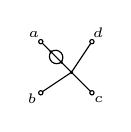
\begin{tikzpicture}[x=0.340cm, y=0.340cm, line width=0.420pt, baseline={([yshift=-0.6ex]0,0)}]
  \draw (-0.955,0.955) -- (-0.573,0.573);
  \draw (-0.955,-0.955) -- (0.191,-0.191);
  \draw (0.955,-0.955) -- (0.191,-0.191);
  \draw (0.955,0.955) -- (0.191,-0.191);
  \draw (-0.573,0.573) arc[start angle=141.026, end angle=308.974, radius=0.271];
  \draw (-0.573,0.573) -- (-0.191,0.191);
  \draw (-0.573,0.573) arc[start angle=128.974, end angle=-38.974, radius=0.271];
  \draw (-0.191,0.191) -- (0.191,-0.191);
  \fill (-0.573,0.573) circle (0.064);
  \fill (-0.191,0.191) circle (0.064);
  \fill (0.191,-0.191) circle (0.064);
  \draw[fill=white] (-0.955,0.955) circle (0.080);
  \draw[fill=white] (-0.955,-0.955) circle (0.080);
  \draw[fill=white] (0.955,-0.955) circle (0.080);
  \draw[fill=white] (0.955,0.955) circle (0.080);
  \node[font=\tiny, inner sep=0pt, anchor=315] at (-1.075,1.075) {$a$};
  \node[font=\tiny, inner sep=0pt, anchor=34] at (-1.096,-1.049) {$b$};
  \node[font=\tiny, inner sep=0pt, anchor=135] at (1.075,-1.075) {$c$};
  \node[font=\tiny, inner sep=0pt, anchor=236] at (1.049,1.096) {$d$};
\end{tikzpicture}}
\diagramgap
\mbox{$\displaystyle +\,\frac{1}{2}$\,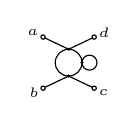
\begin{tikzpicture}[x=0.340cm, y=0.340cm, line width=0.420pt, baseline={([yshift=-0.6ex]0,0)}]
  \draw (-0.955,0.955) -- (0.000,0.500);
  \draw (-0.955,-0.955) -- (0.000,-0.500);
  \draw (0.955,-0.955) -- (0.000,-0.500);
  \draw (0.955,0.955) -- (0.000,0.500);
  \draw (0.500,0.000) arc[start angle=360.000, end angle=450.000, radius=0.500];
  \draw (0.500,0.000) arc[start angle=360.000, end angle=270.000, radius=0.500];
  \draw (0.000,0.500) arc[start angle=90.000, end angle=270.000, radius=0.500];
  \draw (0.500,0.000) arc[start angle=180.000, end angle=540.000, radius=0.280];
  \fill (0.500,0.000) circle (0.064);
  \fill (0.000,0.500) circle (0.064);
  \fill (0.000,-0.500) circle (0.064);
  \draw[fill=white] (-0.955,0.955) circle (0.080);
  \draw[fill=white] (-0.955,-0.955) circle (0.080);
  \draw[fill=white] (0.955,-0.955) circle (0.080);
  \draw[fill=white] (0.955,0.955) circle (0.080);
  \node[font=\tiny, inner sep=0pt, anchor=335] at (-1.108,1.028) {$a$};
  \node[font=\tiny, inner sep=0pt, anchor=25] at (-1.108,-1.028) {$b$};
  \node[font=\tiny, inner sep=0pt, anchor=155] at (1.108,-1.028) {$c$};
  \node[font=\tiny, inner sep=0pt, anchor=205] at (1.108,1.028) {$d$};
\end{tikzpicture}}
\diagramgap
\mbox{$\displaystyle +\,\frac{1}{2}$\,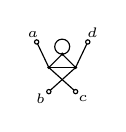
\begin{tikzpicture}[x=0.340cm, y=0.340cm, line width=0.420pt, baseline={([yshift=-0.6ex]0,0)}]
  \draw (-0.955,0.955) -- (-0.500,0.000);
  \draw (-0.500,-0.900) -- (0.500,0.000);
  \draw (0.500,-0.900) -- (-0.500,0.000);
  \draw (0.955,0.955) -- (0.500,0.000);
  \draw (0.000,0.500) -- (-0.500,0.000);
  \draw (0.000,0.500) -- (0.500,0.000);
  \draw (-0.500,0.000) -- (0.500,0.000);
  \draw (0.000,0.500) arc[start angle=270.000, end angle=630.000, radius=0.280];
  \fill (0.000,0.500) circle (0.064);
  \fill (-0.500,0.000) circle (0.064);
  \fill (0.500,0.000) circle (0.064);
  \draw[fill=white] (-0.955,0.955) circle (0.080);
  \draw[fill=white] (-0.500,-0.900) circle (0.080);
  \draw[fill=white] (0.500,-0.900) circle (0.080);
  \draw[fill=white] (0.955,0.955) circle (0.080);
  \node[font=\tiny, inner sep=0pt, anchor=295] at (-1.028,1.108) {$a$};
  \node[font=\tiny, inner sep=0pt, anchor=42] at (-0.626,-1.014) {$b$};
  \node[font=\tiny, inner sep=0pt, anchor=138] at (0.626,-1.014) {$c$};
  \node[font=\tiny, inner sep=0pt, anchor=245] at (1.028,1.108) {$d$};
\end{tikzpicture}}
\diagramgap
\mbox{$\displaystyle +\,\frac{1}{2}$\,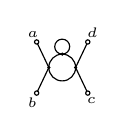
\begin{tikzpicture}[x=0.340cm, y=0.340cm, line width=0.420pt, baseline={([yshift=-0.6ex]0,0)}]
  \draw (-0.955,0.955) -- (-0.500,0.000);
  \draw (-0.955,-0.955) -- (-0.500,0.000);
  \draw (0.955,-0.955) -- (0.500,0.000);
  \draw (0.955,0.955) -- (0.500,0.000);
  \draw (0.000,0.500) arc[start angle=90.000, end angle=180.000, radius=0.500];
  \draw (0.000,0.500) arc[start angle=90.000, end angle=0.000, radius=0.500];
  \draw (-0.500,0.000) arc[start angle=180.000, end angle=360.000, radius=0.500];
  \draw (0.000,0.500) arc[start angle=270.000, end angle=630.000, radius=0.280];
  \fill (0.000,0.500) circle (0.064);
  \fill (-0.500,0.000) circle (0.064);
  \fill (0.500,0.000) circle (0.064);
  \draw[fill=white] (-0.955,0.955) circle (0.080);
  \draw[fill=white] (-0.955,-0.955) circle (0.080);
  \draw[fill=white] (0.955,-0.955) circle (0.080);
  \draw[fill=white] (0.955,0.955) circle (0.080);
  \node[font=\tiny, inner sep=0pt, anchor=295] at (-1.028,1.108) {$a$};
  \node[font=\tiny, inner sep=0pt, anchor=65] at (-1.028,-1.108) {$b$};
  \node[font=\tiny, inner sep=0pt, anchor=115] at (1.028,-1.108) {$c$};
  \node[font=\tiny, inner sep=0pt, anchor=245] at (1.028,1.108) {$d$};
\end{tikzpicture}}
\diagramgap
\mbox{$\displaystyle +\,\frac{1}{2}$\,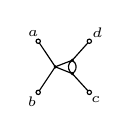
\begin{tikzpicture}[x=0.340cm, y=0.340cm, line width=0.420pt, baseline={([yshift=-0.6ex]0,0)}]
  \draw (-0.955,0.955) -- (-0.318,0.000);
  \draw (-0.955,-0.955) -- (-0.318,0.000);
  \draw (0.955,-0.955) -- (0.318,-0.255);
  \draw (0.955,0.955) -- (0.318,0.245);
  \draw (0.318,-0.255) arc[start angle=300.420, end angle=419.580, radius=0.290];
  \draw (0.318,-0.255) arc[start angle=239.580, end angle=120.420, radius=0.290];
  \draw (0.318,-0.255) -- (-0.318,0.000);
  \draw (0.318,0.245) -- (-0.318,0.000);
  \fill (0.318,-0.255) circle (0.064);
  \fill (0.318,0.245) circle (0.064);
  \fill (-0.318,0.000) circle (0.064);
  \draw[fill=white] (-0.955,0.955) circle (0.080);
  \draw[fill=white] (-0.955,-0.955) circle (0.080);
  \draw[fill=white] (0.955,-0.955) circle (0.080);
  \draw[fill=white] (0.955,0.955) circle (0.080);
  \node[font=\tiny, inner sep=0pt, anchor=304] at (-1.049,1.096) {$a$};
  \node[font=\tiny, inner sep=0pt, anchor=56] at (-1.049,-1.096) {$b$};
  \node[font=\tiny, inner sep=0pt, anchor=132] at (1.069,-1.080) {$c$};
  \node[font=\tiny, inner sep=0pt, anchor=228] at (1.068,1.081) {$d$};
\end{tikzpicture}}
\diagramgap
\mbox{$\displaystyle +\,\frac{1}{2}$\,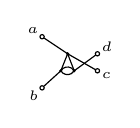
\begin{tikzpicture}[x=0.340cm, y=0.340cm, line width=0.420pt, baseline={([yshift=-0.6ex]0,0)}]
  \draw (-0.955,0.955) -- (0.000,0.318);
  \draw (-0.955,-0.955) -- (-0.255,-0.318);
  \draw (1.113,-0.318) -- (0.000,0.318);
  \draw (1.113,0.318) -- (0.245,-0.318);
  \draw (-0.255,-0.318) arc[start angle=210.420, end angle=329.580, radius=0.290];
  \draw (-0.255,-0.318) arc[start angle=149.580, end angle=30.420, radius=0.290];
  \draw (-0.255,-0.318) -- (0.000,0.318);
  \draw (0.245,-0.318) -- (0.000,0.318);
  \fill (-0.255,-0.318) circle (0.064);
  \fill (0.245,-0.318) circle (0.064);
  \fill (0.000,0.318) circle (0.064);
  \draw[fill=white] (-0.955,0.955) circle (0.080);
  \draw[fill=white] (-0.955,-0.955) circle (0.080);
  \draw[fill=white] (1.113,-0.318) circle (0.080);
  \draw[fill=white] (1.113,0.318) circle (0.080);
  \node[font=\tiny, inner sep=0pt, anchor=326] at (-1.096,1.049) {$a$};
  \node[font=\tiny, inner sep=0pt, anchor=42] at (-1.080,-1.069) {$b$};
  \node[font=\tiny, inner sep=0pt, anchor=150] at (1.260,-0.403) {$c$};
  \node[font=\tiny, inner sep=0pt, anchor=216] at (1.250,0.419) {$d$};
\end{tikzpicture}}
\diagramgap
\mbox{$\displaystyle +\,\frac{1}{2}$\,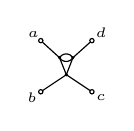
\begin{tikzpicture}[x=0.340cm, y=0.340cm, line width=0.420pt, baseline={([yshift=-0.6ex]0,0)}]
  \draw (-0.955,0.955) -- (-0.255,0.318);
  \draw (-0.955,-0.955) -- (0.000,-0.318);
  \draw (0.955,-0.955) -- (0.000,-0.318);
  \draw (0.955,0.955) -- (0.245,0.318);
  \draw (-0.255,0.318) arc[start angle=210.420, end angle=329.580, radius=0.290];
  \draw (-0.255,0.318) arc[start angle=149.580, end angle=30.420, radius=0.290];
  \draw (-0.255,0.318) -- (0.000,-0.318);
  \draw (0.245,0.318) -- (0.000,-0.318);
  \fill (-0.255,0.318) circle (0.064);
  \fill (0.245,0.318) circle (0.064);
  \fill (0.000,-0.318) circle (0.064);
  \draw[fill=white] (-0.955,0.955) circle (0.080);
  \draw[fill=white] (-0.955,-0.955) circle (0.080);
  \draw[fill=white] (0.955,-0.955) circle (0.080);
  \draw[fill=white] (0.955,0.955) circle (0.080);
  \node[font=\tiny, inner sep=0pt, anchor=318] at (-1.080,1.069) {$a$};
  \node[font=\tiny, inner sep=0pt, anchor=34] at (-1.096,-1.049) {$b$};
  \node[font=\tiny, inner sep=0pt, anchor=146] at (1.096,-1.049) {$c$};
  \node[font=\tiny, inner sep=0pt, anchor=222] at (1.081,1.068) {$d$};
\end{tikzpicture}}
\diagramgap
\mbox{$\displaystyle +\,\frac{1}{2}$\,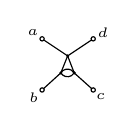
\begin{tikzpicture}[x=0.340cm, y=0.340cm, line width=0.420pt, baseline={([yshift=-0.6ex]0,0)}]
  \draw (-0.955,0.955) -- (0.000,0.318);
  \draw (-0.955,-0.955) -- (-0.255,-0.318);
  \draw (0.955,-0.955) -- (0.245,-0.318);
  \draw (0.955,0.955) -- (0.000,0.318);
  \draw (-0.255,-0.318) arc[start angle=210.420, end angle=329.580, radius=0.290];
  \draw (-0.255,-0.318) arc[start angle=149.580, end angle=30.420, radius=0.290];
  \draw (-0.255,-0.318) -- (0.000,0.318);
  \draw (0.245,-0.318) -- (0.000,0.318);
  \fill (-0.255,-0.318) circle (0.064);
  \fill (0.245,-0.318) circle (0.064);
  \fill (0.000,0.318) circle (0.064);
  \draw[fill=white] (-0.955,0.955) circle (0.080);
  \draw[fill=white] (-0.955,-0.955) circle (0.080);
  \draw[fill=white] (0.955,-0.955) circle (0.080);
  \draw[fill=white] (0.955,0.955) circle (0.080);
  \node[font=\tiny, inner sep=0pt, anchor=326] at (-1.096,1.049) {$a$};
  \node[font=\tiny, inner sep=0pt, anchor=42] at (-1.080,-1.069) {$b$};
  \node[font=\tiny, inner sep=0pt, anchor=138] at (1.081,-1.068) {$c$};
  \node[font=\tiny, inner sep=0pt, anchor=214] at (1.096,1.049) {$d$};
\end{tikzpicture}}
\diagramgap
\mbox{$\displaystyle +\,\frac{1}{2}$\,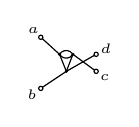
\begin{tikzpicture}[x=0.340cm, y=0.340cm, line width=0.420pt, baseline={([yshift=-0.6ex]0,0)}]
  \draw (-0.955,0.955) -- (-0.255,0.318);
  \draw (-0.955,-0.955) -- (0.000,-0.318);
  \draw (1.113,-0.318) -- (0.245,0.318);
  \draw (1.113,0.318) -- (0.000,-0.318);
  \draw (-0.255,0.318) arc[start angle=210.420, end angle=329.580, radius=0.290];
  \draw (-0.255,0.318) arc[start angle=149.580, end angle=30.420, radius=0.290];
  \draw (-0.255,0.318) -- (0.000,-0.318);
  \draw (0.245,0.318) -- (0.000,-0.318);
  \fill (-0.255,0.318) circle (0.064);
  \fill (0.245,0.318) circle (0.064);
  \fill (0.000,-0.318) circle (0.064);
  \draw[fill=white] (-0.955,0.955) circle (0.080);
  \draw[fill=white] (-0.955,-0.955) circle (0.080);
  \draw[fill=white] (1.113,-0.318) circle (0.080);
  \draw[fill=white] (1.113,0.318) circle (0.080);
  \node[font=\tiny, inner sep=0pt, anchor=318] at (-1.080,1.069) {$a$};
  \node[font=\tiny, inner sep=0pt, anchor=34] at (-1.096,-1.049) {$b$};
  \node[font=\tiny, inner sep=0pt, anchor=144] at (1.250,-0.419) {$c$};
  \node[font=\tiny, inner sep=0pt, anchor=210] at (1.260,0.403) {$d$};
\end{tikzpicture}}
\diagramgap
\mbox{$\displaystyle +\,\frac{1}{2}$\,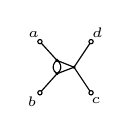
\begin{tikzpicture}[x=0.340cm, y=0.340cm, line width=0.420pt, baseline={([yshift=-0.6ex]0,0)}]
  \draw (-0.955,0.955) -- (-0.318,0.255);
  \draw (-0.955,-0.955) -- (-0.318,-0.245);
  \draw (0.955,-0.955) -- (0.318,0.000);
  \draw (0.955,0.955) -- (0.318,0.000);
  \draw (-0.318,0.255) arc[start angle=120.420, end angle=239.580, radius=0.290];
  \draw (-0.318,0.255) arc[start angle=59.580, end angle=-59.580, radius=0.290];
  \draw (-0.318,0.255) -- (0.318,0.000);
  \draw (-0.318,-0.245) -- (0.318,0.000);
  \fill (-0.318,0.255) circle (0.064);
  \fill (-0.318,-0.245) circle (0.064);
  \fill (0.318,0.000) circle (0.064);
  \draw[fill=white] (-0.955,0.955) circle (0.080);
  \draw[fill=white] (-0.955,-0.955) circle (0.080);
  \draw[fill=white] (0.955,-0.955) circle (0.080);
  \draw[fill=white] (0.955,0.955) circle (0.080);
  \node[font=\tiny, inner sep=0pt, anchor=312] at (-1.069,1.080) {$a$};
  \node[font=\tiny, inner sep=0pt, anchor=48] at (-1.068,-1.081) {$b$};
  \node[font=\tiny, inner sep=0pt, anchor=124] at (1.049,-1.096) {$c$};
  \node[font=\tiny, inner sep=0pt, anchor=236] at (1.049,1.096) {$d$};
\end{tikzpicture}}
\diagramgap
\mbox{$\displaystyle +\,\frac{1}{4}$\,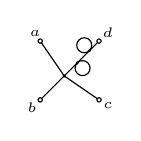
\begin{tikzpicture}[x=0.340cm, y=0.340cm, line width=0.420pt, baseline={([yshift=-0.6ex]0,0)}]
  \draw (-1.098,1.098) -- (-0.203,-0.203);
  \draw (-1.098,-1.098) -- (-0.203,-0.203);
  \draw (1.098,-1.098) -- (-0.203,-0.203);
  \draw (1.098,1.098) -- (0.744,0.744);
  \draw (0.744,0.744) -- (0.285,0.285);
  \draw (0.285,0.285) -- (-0.203,-0.203);
  \draw (0.744,0.744) arc[start angle=315.000, end angle=675.000, radius=0.280];
  \draw (0.285,0.285) arc[start angle=135.000, end angle=495.000, radius=0.280];
  \fill (0.744,0.744) circle (0.064);
  \fill (0.285,0.285) circle (0.064);
  \fill (-0.203,-0.203) circle (0.064);
  \draw[fill=white] (-1.098,1.098) circle (0.080);
  \draw[fill=white] (-1.098,-1.098) circle (0.080);
  \draw[fill=white] (1.098,-1.098) circle (0.080);
  \draw[fill=white] (1.098,1.098) circle (0.080);
  \node[font=\tiny, inner sep=0pt, anchor=305] at (-1.194,1.238) {$a$};
  \node[font=\tiny, inner sep=0pt, anchor=45] at (-1.218,-1.218) {$b$};
  \node[font=\tiny, inner sep=0pt, anchor=145] at (1.238,-1.194) {$c$};
  \node[font=\tiny, inner sep=0pt, anchor=225] at (1.218,1.218) {$d$};
\end{tikzpicture}}
\diagramgap
\mbox{$\displaystyle +\,\frac{1}{4}$\,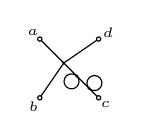
\begin{tikzpicture}[x=0.340cm, y=0.340cm, line width=0.420pt, baseline={([yshift=-0.6ex]0,0)}]
  \draw (-1.098,1.098) -- (-0.203,0.203);
  \draw (-1.098,-1.098) -- (-0.203,0.203);
  \draw (1.098,-1.098) -- (0.744,-0.744);
  \draw (1.098,1.098) -- (-0.203,0.203);
  \draw (0.744,-0.744) -- (0.285,-0.285);
  \draw (0.285,-0.285) -- (-0.203,0.203);
  \draw (0.744,-0.744) arc[start angle=225.000, end angle=585.000, radius=0.280];
  \draw (0.285,-0.285) arc[start angle=45.000, end angle=405.000, radius=0.280];
  \fill (0.744,-0.744) circle (0.064);
  \fill (0.285,-0.285) circle (0.064);
  \fill (-0.203,0.203) circle (0.064);
  \draw[fill=white] (-1.098,1.098) circle (0.080);
  \draw[fill=white] (-1.098,-1.098) circle (0.080);
  \draw[fill=white] (1.098,-1.098) circle (0.080);
  \draw[fill=white] (1.098,1.098) circle (0.080);
  \node[font=\tiny, inner sep=0pt, anchor=315] at (-1.218,1.218) {$a$};
  \node[font=\tiny, inner sep=0pt, anchor=55] at (-1.194,-1.238) {$b$};
  \node[font=\tiny, inner sep=0pt, anchor=135] at (1.218,-1.218) {$c$};
  \node[font=\tiny, inner sep=0pt, anchor=215] at (1.238,1.194) {$d$};
\end{tikzpicture}}
\diagramgap
\mbox{$\displaystyle +\,\frac{1}{4}$\,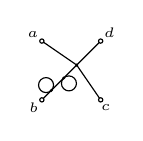
\begin{tikzpicture}[x=0.340cm, y=0.340cm, line width=0.420pt, baseline={([yshift=-0.6ex]0,0)}]
  \draw (-1.098,1.098) -- (0.203,0.203);
  \draw (-1.098,-1.098) -- (-0.744,-0.744);
  \draw (1.098,-1.098) -- (0.203,0.203);
  \draw (1.098,1.098) -- (0.203,0.203);
  \draw (-0.744,-0.744) -- (-0.285,-0.285);
  \draw (-0.285,-0.285) -- (0.203,0.203);
  \draw (-0.744,-0.744) arc[start angle=315.000, end angle=675.000, radius=0.280];
  \draw (-0.285,-0.285) arc[start angle=135.000, end angle=495.000, radius=0.280];
  \fill (-0.744,-0.744) circle (0.064);
  \fill (-0.285,-0.285) circle (0.064);
  \fill (0.203,0.203) circle (0.064);
  \draw[fill=white] (-1.098,1.098) circle (0.080);
  \draw[fill=white] (-1.098,-1.098) circle (0.080);
  \draw[fill=white] (1.098,-1.098) circle (0.080);
  \draw[fill=white] (1.098,1.098) circle (0.080);
  \node[font=\tiny, inner sep=0pt, anchor=325] at (-1.238,1.194) {$a$};
  \node[font=\tiny, inner sep=0pt, anchor=45] at (-1.218,-1.218) {$b$};
  \node[font=\tiny, inner sep=0pt, anchor=125] at (1.194,-1.238) {$c$};
  \node[font=\tiny, inner sep=0pt, anchor=225] at (1.218,1.218) {$d$};
\end{tikzpicture}}
\diagramgap
\mbox{$\displaystyle +\,\frac{1}{4}$\,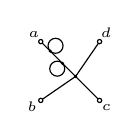
\begin{tikzpicture}[x=0.340cm, y=0.340cm, line width=0.420pt, baseline={([yshift=-0.6ex]0,0)}]
  \draw (-1.098,1.098) -- (-0.744,0.744);
  \draw (-1.098,-1.098) -- (0.203,-0.203);
  \draw (1.098,-1.098) -- (0.203,-0.203);
  \draw (1.098,1.098) -- (0.203,-0.203);
  \draw (-0.744,0.744) -- (-0.285,0.285);
  \draw (-0.285,0.285) -- (0.203,-0.203);
  \draw (-0.744,0.744) arc[start angle=225.000, end angle=585.000, radius=0.280];
  \draw (-0.285,0.285) arc[start angle=45.000, end angle=405.000, radius=0.280];
  \fill (-0.744,0.744) circle (0.064);
  \fill (-0.285,0.285) circle (0.064);
  \fill (0.203,-0.203) circle (0.064);
  \draw[fill=white] (-1.098,1.098) circle (0.080);
  \draw[fill=white] (-1.098,-1.098) circle (0.080);
  \draw[fill=white] (1.098,-1.098) circle (0.080);
  \draw[fill=white] (1.098,1.098) circle (0.080);
  \node[font=\tiny, inner sep=0pt, anchor=315] at (-1.218,1.218) {$a$};
  \node[font=\tiny, inner sep=0pt, anchor=35] at (-1.238,-1.194) {$b$};
  \node[font=\tiny, inner sep=0pt, anchor=135] at (1.218,-1.218) {$c$};
  \node[font=\tiny, inner sep=0pt, anchor=235] at (1.194,1.238) {$d$};
\end{tikzpicture}}
\diagramgap
\mbox{$\displaystyle +\,\frac{1}{4}$\,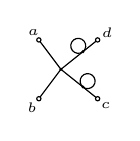
\begin{tikzpicture}[x=0.340cm, y=0.340cm, line width=0.420pt, baseline={([yshift=-0.6ex]0,0)}]
  \draw (-1.098,1.098) -- (-0.274,0.000);
  \draw (-1.098,-1.098) -- (-0.274,0.000);
  \draw (1.098,-1.098) -- (0.549,-0.659);
  \draw (1.098,1.098) -- (0.549,0.659);
  \draw (0.549,-0.659) -- (-0.274,0.000);
  \draw (0.549,0.659) -- (-0.274,0.000);
  \draw (0.549,-0.659) arc[start angle=231.340, end angle=591.340, radius=0.280];
  \draw (0.549,0.659) arc[start angle=308.660, end angle=668.660, radius=0.280];
  \fill (0.549,-0.659) circle (0.064);
  \fill (0.549,0.659) circle (0.064);
  \fill (-0.274,0.000) circle (0.064);
  \draw[fill=white] (-1.098,1.098) circle (0.080);
  \draw[fill=white] (-1.098,-1.098) circle (0.080);
  \draw[fill=white] (1.098,-1.098) circle (0.080);
  \draw[fill=white] (1.098,1.098) circle (0.080);
  \node[font=\tiny, inner sep=0pt, anchor=307] at (-1.200,1.234) {$a$};
  \node[font=\tiny, inner sep=0pt, anchor=53] at (-1.200,-1.234) {$b$};
  \node[font=\tiny, inner sep=0pt, anchor=141] at (1.231,-1.204) {$c$};
  \node[font=\tiny, inner sep=0pt, anchor=219] at (1.231,1.204) {$d$};
\end{tikzpicture}}
\diagramgap
\mbox{$\displaystyle +\,\frac{1}{4}$\,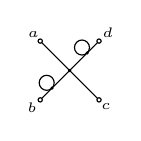
\begin{tikzpicture}[x=0.340cm, y=0.340cm, line width=0.420pt, baseline={([yshift=-0.6ex]0,0)}]
  \draw (-1.098,1.098) -- (0.000,0.000);
  \draw (-1.098,-1.098) -- (-0.659,-0.659);
  \draw (1.098,-1.098) -- (0.000,0.000);
  \draw (1.098,1.098) -- (0.659,0.659);
  \draw (-0.659,-0.659) -- (0.000,0.000);
  \draw (0.659,0.659) -- (0.000,0.000);
  \draw (-0.659,-0.659) arc[start angle=315.000, end angle=675.000, radius=0.280];
  \draw (0.659,0.659) arc[start angle=315.000, end angle=675.000, radius=0.280];
  \fill (-0.659,-0.659) circle (0.064);
  \fill (0.659,0.659) circle (0.064);
  \fill (0.000,0.000) circle (0.064);
  \draw[fill=white] (-1.098,1.098) circle (0.080);
  \draw[fill=white] (-1.098,-1.098) circle (0.080);
  \draw[fill=white] (1.098,-1.098) circle (0.080);
  \draw[fill=white] (1.098,1.098) circle (0.080);
  \node[font=\tiny, inner sep=0pt, anchor=315] at (-1.218,1.218) {$a$};
  \node[font=\tiny, inner sep=0pt, anchor=45] at (-1.218,-1.218) {$b$};
  \node[font=\tiny, inner sep=0pt, anchor=135] at (1.218,-1.218) {$c$};
  \node[font=\tiny, inner sep=0pt, anchor=225] at (1.218,1.218) {$d$};
\end{tikzpicture}}
\diagramgap
\mbox{$\displaystyle +\,\frac{1}{4}$\,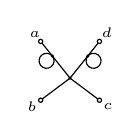
\begin{tikzpicture}[x=0.340cm, y=0.340cm, line width=0.420pt, baseline={([yshift=-0.6ex]0,0)}]
  \draw (-1.098,1.098) -- (-0.659,0.549);
  \draw (-1.098,-1.098) -- (0.000,-0.274);
  \draw (1.098,-1.098) -- (0.000,-0.274);
  \draw (1.098,1.098) -- (0.659,0.549);
  \draw (-0.659,0.549) -- (0.000,-0.274);
  \draw (0.659,0.549) -- (0.000,-0.274);
  \draw (-0.659,0.549) arc[start angle=38.660, end angle=398.660, radius=0.280];
  \draw (0.659,0.549) arc[start angle=141.340, end angle=501.340, radius=0.280];
  \fill (-0.659,0.549) circle (0.064);
  \fill (0.659,0.549) circle (0.064);
  \fill (0.000,-0.274) circle (0.064);
  \draw[fill=white] (-1.098,1.098) circle (0.080);
  \draw[fill=white] (-1.098,-1.098) circle (0.080);
  \draw[fill=white] (1.098,-1.098) circle (0.080);
  \draw[fill=white] (1.098,1.098) circle (0.080);
  \node[font=\tiny, inner sep=0pt, anchor=309] at (-1.204,1.231) {$a$};
  \node[font=\tiny, inner sep=0pt, anchor=37] at (-1.234,-1.200) {$b$};
  \node[font=\tiny, inner sep=0pt, anchor=143] at (1.234,-1.200) {$c$};
  \node[font=\tiny, inner sep=0pt, anchor=231] at (1.204,1.231) {$d$};
\end{tikzpicture}}
\diagramgap
\mbox{$\displaystyle +\,\frac{1}{4}$\,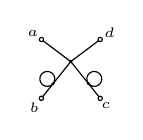
\begin{tikzpicture}[x=0.340cm, y=0.340cm, line width=0.420pt, baseline={([yshift=-0.6ex]0,0)}]
  \draw (-1.098,1.098) -- (0.000,0.274);
  \draw (-1.098,-1.098) -- (-0.659,-0.549);
  \draw (1.098,-1.098) -- (0.659,-0.549);
  \draw (1.098,1.098) -- (0.000,0.274);
  \draw (-0.659,-0.549) -- (0.000,0.274);
  \draw (0.659,-0.549) -- (0.000,0.274);
  \draw (-0.659,-0.549) arc[start angle=321.340, end angle=681.340, radius=0.280];
  \draw (0.659,-0.549) arc[start angle=218.660, end angle=578.660, radius=0.280];
  \fill (-0.659,-0.549) circle (0.064);
  \fill (0.659,-0.549) circle (0.064);
  \fill (0.000,0.274) circle (0.064);
  \draw[fill=white] (-1.098,1.098) circle (0.080);
  \draw[fill=white] (-1.098,-1.098) circle (0.080);
  \draw[fill=white] (1.098,-1.098) circle (0.080);
  \draw[fill=white] (1.098,1.098) circle (0.080);
  \node[font=\tiny, inner sep=0pt, anchor=323] at (-1.234,1.200) {$a$};
  \node[font=\tiny, inner sep=0pt, anchor=51] at (-1.204,-1.231) {$b$};
  \node[font=\tiny, inner sep=0pt, anchor=129] at (1.204,-1.231) {$c$};
  \node[font=\tiny, inner sep=0pt, anchor=217] at (1.234,1.200) {$d$};
\end{tikzpicture}}
\diagramgap
\mbox{$\displaystyle +\,\frac{1}{4}$\,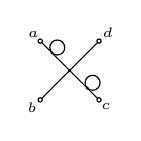
\begin{tikzpicture}[x=0.340cm, y=0.340cm, line width=0.420pt, baseline={([yshift=-0.6ex]0,0)}]
  \draw (-1.098,1.098) -- (-0.659,0.659);
  \draw (-1.098,-1.098) -- (0.000,0.000);
  \draw (1.098,-1.098) -- (0.659,-0.659);
  \draw (1.098,1.098) -- (0.000,0.000);
  \draw (-0.659,0.659) -- (0.000,0.000);
  \draw (0.659,-0.659) -- (0.000,0.000);
  \draw (-0.659,0.659) arc[start angle=225.000, end angle=585.000, radius=0.280];
  \draw (0.659,-0.659) arc[start angle=225.000, end angle=585.000, radius=0.280];
  \fill (-0.659,0.659) circle (0.064);
  \fill (0.659,-0.659) circle (0.064);
  \fill (0.000,0.000) circle (0.064);
  \draw[fill=white] (-1.098,1.098) circle (0.080);
  \draw[fill=white] (-1.098,-1.098) circle (0.080);
  \draw[fill=white] (1.098,-1.098) circle (0.080);
  \draw[fill=white] (1.098,1.098) circle (0.080);
  \node[font=\tiny, inner sep=0pt, anchor=315] at (-1.218,1.218) {$a$};
  \node[font=\tiny, inner sep=0pt, anchor=45] at (-1.218,-1.218) {$b$};
  \node[font=\tiny, inner sep=0pt, anchor=135] at (1.218,-1.218) {$c$};
  \node[font=\tiny, inner sep=0pt, anchor=225] at (1.218,1.218) {$d$};
\end{tikzpicture}}
\diagramgap
\mbox{$\displaystyle +\,\frac{1}{4}$\,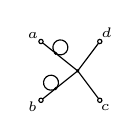
\begin{tikzpicture}[x=0.340cm, y=0.340cm, line width=0.420pt, baseline={([yshift=-0.6ex]0,0)}]
  \draw (-1.098,1.098) -- (-0.549,0.659);
  \draw (-1.098,-1.098) -- (-0.549,-0.659);
  \draw (1.098,-1.098) -- (0.274,0.000);
  \draw (1.098,1.098) -- (0.274,0.000);
  \draw (-0.549,0.659) -- (0.274,0.000);
  \draw (-0.549,-0.659) -- (0.274,0.000);
  \draw (-0.549,0.659) arc[start angle=231.340, end angle=591.340, radius=0.280];
  \draw (-0.549,-0.659) arc[start angle=308.660, end angle=668.660, radius=0.280];
  \fill (-0.549,0.659) circle (0.064);
  \fill (-0.549,-0.659) circle (0.064);
  \fill (0.274,0.000) circle (0.064);
  \draw[fill=white] (-1.098,1.098) circle (0.080);
  \draw[fill=white] (-1.098,-1.098) circle (0.080);
  \draw[fill=white] (1.098,-1.098) circle (0.080);
  \draw[fill=white] (1.098,1.098) circle (0.080);
  \node[font=\tiny, inner sep=0pt, anchor=321] at (-1.231,1.204) {$a$};
  \node[font=\tiny, inner sep=0pt, anchor=39] at (-1.231,-1.204) {$b$};
  \node[font=\tiny, inner sep=0pt, anchor=127] at (1.200,-1.234) {$c$};
  \node[font=\tiny, inner sep=0pt, anchor=233] at (1.200,1.234) {$d$};
\end{tikzpicture}}
\diagramgap
\mbox{$\displaystyle +\,\frac{1}{4}$\,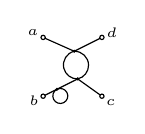
\begin{tikzpicture}[x=0.340cm, y=0.340cm, line width=0.420pt, baseline={([yshift=-0.6ex]0,0)}]
  \draw (-1.098,1.098) -- (0.065,0.581);
  \draw (-1.098,-1.098) -- (-0.581,-0.839);
  \draw (1.098,-1.098) -- (0.194,-0.452);
  \draw (1.098,1.098) -- (0.065,0.581);
  \draw (0.065,0.581) arc[start angle=103.151, end angle=271.099, radius=0.524];
  \draw (0.065,0.581) arc[start angle=91.099, end angle=-76.849, radius=0.524];
  \draw (-0.581,-0.839) -- (0.194,-0.452);
  \draw (-0.581,-0.839) arc[start angle=116.565, end angle=476.565, radius=0.280];
  \fill (0.065,0.581) circle (0.064);
  \fill (-0.581,-0.839) circle (0.064);
  \fill (0.194,-0.452) circle (0.064);
  \draw[fill=white] (-1.098,1.098) circle (0.080);
  \draw[fill=white] (-1.098,-1.098) circle (0.080);
  \draw[fill=white] (1.098,-1.098) circle (0.080);
  \draw[fill=white] (1.098,1.098) circle (0.080);
  \node[font=\tiny, inner sep=0pt, anchor=336] at (-1.253,1.167) {$a$};
  \node[font=\tiny, inner sep=0pt, anchor=27] at (-1.250,-1.174) {$b$};
  \node[font=\tiny, inner sep=0pt, anchor=144] at (1.236,-1.197) {$c$};
  \node[font=\tiny, inner sep=0pt, anchor=207] at (1.250,1.174) {$d$};
\end{tikzpicture}}
\diagramgap
\mbox{$\displaystyle +\,\frac{1}{4}$\,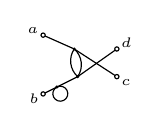
\begin{tikzpicture}[x=0.340cm, y=0.340cm, line width=0.420pt, baseline={([yshift=-0.6ex]0,0)}]
  \draw (-1.098,1.098) -- (0.065,0.581);
  \draw (-1.098,-1.098) -- (-0.581,-0.839);
  \draw (1.656,-0.452) -- (0.065,0.581);
  \draw (1.656,0.581) -- (0.194,-0.452);
  \draw (0.065,0.581) arc[start angle=145.832, end angle=228.418, radius=0.789];
  \draw (0.065,0.581) arc[start angle=48.418, end angle=-34.168, radius=0.789];
  \draw (-0.581,-0.839) -- (0.194,-0.452);
  \draw (-0.581,-0.839) arc[start angle=116.565, end angle=476.565, radius=0.280];
  \fill (0.065,0.581) circle (0.064);
  \fill (-0.581,-0.839) circle (0.064);
  \fill (0.194,-0.452) circle (0.064);
  \draw[fill=white] (-1.098,1.098) circle (0.080);
  \draw[fill=white] (-1.098,-1.098) circle (0.080);
  \draw[fill=white] (1.656,-0.452) circle (0.080);
  \draw[fill=white] (1.656,0.581) circle (0.080);
  \node[font=\tiny, inner sep=0pt, anchor=336] at (-1.253,1.167) {$a$};
  \node[font=\tiny, inner sep=0pt, anchor=27] at (-1.250,-1.174) {$b$};
  \node[font=\tiny, inner sep=0pt, anchor=147] at (1.799,-0.545) {$c$};
  \node[font=\tiny, inner sep=0pt, anchor=215] at (1.795,0.679) {$d$};
\end{tikzpicture}}
\diagramgap
\mbox{$\displaystyle +\,\frac{1}{4}$\,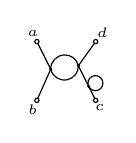
\begin{tikzpicture}[x=0.340cm, y=0.340cm, line width=0.420pt, baseline={([yshift=-0.6ex]0,0)}]
  \draw (-1.098,1.098) -- (-0.581,0.065);
  \draw (-1.098,-1.098) -- (-0.581,0.065);
  \draw (1.098,-1.098) -- (0.839,-0.581);
  \draw (1.098,1.098) -- (0.452,0.194);
  \draw (-0.581,0.065) arc[start angle=193.151, end angle=361.099, radius=0.524];
  \draw (-0.581,0.065) arc[start angle=181.099, end angle=13.151, radius=0.524];
  \draw (0.839,-0.581) -- (0.452,0.194);
  \draw (0.839,-0.581) arc[start angle=206.565, end angle=566.565, radius=0.280];
  \fill (-0.581,0.065) circle (0.064);
  \fill (0.839,-0.581) circle (0.064);
  \fill (0.452,0.194) circle (0.064);
  \draw[fill=white] (-1.098,1.098) circle (0.080);
  \draw[fill=white] (-1.098,-1.098) circle (0.080);
  \draw[fill=white] (1.098,-1.098) circle (0.080);
  \draw[fill=white] (1.098,1.098) circle (0.080);
  \node[font=\tiny, inner sep=0pt, anchor=297] at (-1.174,1.250) {$a$};
  \node[font=\tiny, inner sep=0pt, anchor=66] at (-1.167,-1.253) {$b$};
  \node[font=\tiny, inner sep=0pt, anchor=117] at (1.174,-1.250) {$c$};
  \node[font=\tiny, inner sep=0pt, anchor=234] at (1.197,1.236) {$d$};
\end{tikzpicture}}
\diagramgap
\mbox{$\displaystyle +\,\frac{1}{4}$\,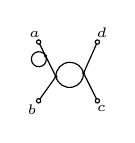
\begin{tikzpicture}[x=0.340cm, y=0.340cm, line width=0.420pt, baseline={([yshift=-0.6ex]0,0)}]
  \draw (-1.098,1.098) -- (-0.839,0.581);
  \draw (-1.098,-1.098) -- (-0.452,-0.194);
  \draw (1.098,-1.098) -- (0.581,-0.065);
  \draw (1.098,1.098) -- (0.581,-0.065);
  \draw (-0.839,0.581) -- (-0.452,-0.194);
  \draw (-0.452,-0.194) arc[start angle=193.151, end angle=361.099, radius=0.524];
  \draw (-0.452,-0.194) arc[start angle=181.099, end angle=13.151, radius=0.524];
  \draw (-0.839,0.581) arc[start angle=26.565, end angle=386.565, radius=0.280];
  \fill (-0.839,0.581) circle (0.064);
  \fill (-0.452,-0.194) circle (0.064);
  \fill (0.581,-0.065) circle (0.064);
  \draw[fill=white] (-1.098,1.098) circle (0.080);
  \draw[fill=white] (-1.098,-1.098) circle (0.080);
  \draw[fill=white] (1.098,-1.098) circle (0.080);
  \draw[fill=white] (1.098,1.098) circle (0.080);
  \node[font=\tiny, inner sep=0pt, anchor=297] at (-1.174,1.250) {$a$};
  \node[font=\tiny, inner sep=0pt, anchor=54] at (-1.197,-1.236) {$b$};
  \node[font=\tiny, inner sep=0pt, anchor=117] at (1.174,-1.250) {$c$};
  \node[font=\tiny, inner sep=0pt, anchor=246] at (1.167,1.253) {$d$};
\end{tikzpicture}}
\diagramgap
\mbox{$\displaystyle +\,\frac{1}{4}$\,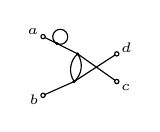
\begin{tikzpicture}[x=0.340cm, y=0.340cm, line width=0.420pt, baseline={([yshift=-0.6ex]0,0)}]
  \draw (-1.098,1.098) -- (-0.581,0.839);
  \draw (-1.098,-1.098) -- (0.065,-0.581);
  \draw (1.656,-0.581) -- (0.194,0.452);
  \draw (1.656,0.452) -- (0.065,-0.581);
  \draw (-0.581,0.839) -- (0.194,0.452);
  \draw (0.065,-0.581) arc[start angle=311.582, end angle=394.168, radius=0.789];
  \draw (0.065,-0.581) arc[start angle=214.168, end angle=131.582, radius=0.789];
  \draw (-0.581,0.839) arc[start angle=243.435, end angle=603.435, radius=0.280];
  \fill (-0.581,0.839) circle (0.064);
  \fill (0.065,-0.581) circle (0.064);
  \fill (0.194,0.452) circle (0.064);
  \draw[fill=white] (-1.098,1.098) circle (0.080);
  \draw[fill=white] (-1.098,-1.098) circle (0.080);
  \draw[fill=white] (1.656,-0.581) circle (0.080);
  \draw[fill=white] (1.656,0.452) circle (0.080);
  \node[font=\tiny, inner sep=0pt, anchor=333] at (-1.250,1.174) {$a$};
  \node[font=\tiny, inner sep=0pt, anchor=24] at (-1.253,-1.167) {$b$};
  \node[font=\tiny, inner sep=0pt, anchor=145] at (1.795,-0.679) {$c$};
  \node[font=\tiny, inner sep=0pt, anchor=213] at (1.799,0.545) {$d$};
\end{tikzpicture}}
\diagramgap
\mbox{$\displaystyle +\,\frac{1}{4}$\,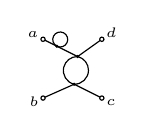
\begin{tikzpicture}[x=0.340cm, y=0.340cm, line width=0.420pt, baseline={([yshift=-0.6ex]0,0)}]
  \draw (-1.098,1.098) -- (-0.581,0.839);
  \draw (-1.098,-1.098) -- (0.065,-0.581);
  \draw (1.098,-1.098) -- (0.065,-0.581);
  \draw (1.098,1.098) -- (0.194,0.452);
  \draw (-0.581,0.839) -- (0.194,0.452);
  \draw (0.065,-0.581) arc[start angle=268.901, end angle=436.849, radius=0.524];
  \draw (0.065,-0.581) arc[start angle=256.849, end angle=88.901, radius=0.524];
  \draw (-0.581,0.839) arc[start angle=243.435, end angle=603.435, radius=0.280];
  \fill (-0.581,0.839) circle (0.064);
  \fill (0.065,-0.581) circle (0.064);
  \fill (0.194,0.452) circle (0.064);
  \draw[fill=white] (-1.098,1.098) circle (0.080);
  \draw[fill=white] (-1.098,-1.098) circle (0.080);
  \draw[fill=white] (1.098,-1.098) circle (0.080);
  \draw[fill=white] (1.098,1.098) circle (0.080);
  \node[font=\tiny, inner sep=0pt, anchor=333] at (-1.250,1.174) {$a$};
  \node[font=\tiny, inner sep=0pt, anchor=24] at (-1.253,-1.167) {$b$};
  \node[font=\tiny, inner sep=0pt, anchor=153] at (1.250,-1.174) {$c$};
  \node[font=\tiny, inner sep=0pt, anchor=216] at (1.236,1.197) {$d$};
\end{tikzpicture}}
\diagramgap
\mbox{$\displaystyle +\,\frac{1}{4}$\,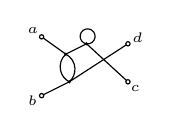
\begin{tikzpicture}[x=0.340cm, y=0.340cm, line width=0.420pt, baseline={([yshift=-0.6ex]0,0)}]
  \draw (-1.098,1.098) -- (-0.194,0.452);
  \draw (-1.098,-1.098) -- (-0.065,-0.581);
  \draw (2.127,-0.581) -- (0.581,0.839);
  \draw (2.127,0.839) -- (-0.065,-0.581);
  \draw (-0.194,0.452) arc[start angle=131.549, end angle=242.701, radius=0.631];
  \draw (-0.194,0.452) arc[start angle=62.701, end angle=-48.451, radius=0.631];
  \draw (-0.194,0.452) -- (0.581,0.839);
  \draw (0.581,0.839) arc[start angle=261.989, end angle=621.989, radius=0.280];
  \fill (-0.194,0.452) circle (0.064);
  \fill (-0.065,-0.581) circle (0.064);
  \fill (0.581,0.839) circle (0.064);
  \draw[fill=white] (-1.098,1.098) circle (0.080);
  \draw[fill=white] (-1.098,-1.098) circle (0.080);
  \draw[fill=white] (2.127,-0.581) circle (0.080);
  \draw[fill=white] (2.127,0.839) circle (0.080);
  \node[font=\tiny, inner sep=0pt, anchor=324] at (-1.236,1.197) {$a$};
  \node[font=\tiny, inner sep=0pt, anchor=27] at (-1.250,-1.174) {$b$};
  \node[font=\tiny, inner sep=0pt, anchor=137] at (2.252,-0.696) {$c$};
  \node[font=\tiny, inner sep=0pt, anchor=213] at (2.270,0.932) {$d$};
\end{tikzpicture}}
\diagramgap
\mbox{$\displaystyle +\,\frac{1}{4}$\,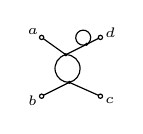
\begin{tikzpicture}[x=0.340cm, y=0.340cm, line width=0.420pt, baseline={([yshift=-0.6ex]0,0)}]
  \draw (-1.098,1.098) -- (-0.194,0.452);
  \draw (-1.098,-1.098) -- (-0.065,-0.581);
  \draw (1.098,-1.098) -- (-0.065,-0.581);
  \draw (1.098,1.098) -- (0.581,0.839);
  \draw (-0.194,0.452) arc[start angle=103.151, end angle=271.099, radius=0.524];
  \draw (-0.194,0.452) arc[start angle=91.099, end angle=-76.849, radius=0.524];
  \draw (-0.194,0.452) -- (0.581,0.839);
  \draw (0.581,0.839) arc[start angle=296.565, end angle=656.565, radius=0.280];
  \fill (-0.194,0.452) circle (0.064);
  \fill (-0.065,-0.581) circle (0.064);
  \fill (0.581,0.839) circle (0.064);
  \draw[fill=white] (-1.098,1.098) circle (0.080);
  \draw[fill=white] (-1.098,-1.098) circle (0.080);
  \draw[fill=white] (1.098,-1.098) circle (0.080);
  \draw[fill=white] (1.098,1.098) circle (0.080);
  \node[font=\tiny, inner sep=0pt, anchor=324] at (-1.236,1.197) {$a$};
  \node[font=\tiny, inner sep=0pt, anchor=27] at (-1.250,-1.174) {$b$};
  \node[font=\tiny, inner sep=0pt, anchor=156] at (1.253,-1.167) {$c$};
  \node[font=\tiny, inner sep=0pt, anchor=207] at (1.250,1.174) {$d$};
\end{tikzpicture}}
\diagramgap
\mbox{$\displaystyle +\,\frac{1}{4}$\,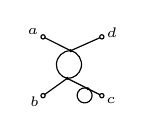
\begin{tikzpicture}[x=0.340cm, y=0.340cm, line width=0.420pt, baseline={([yshift=-0.6ex]0,0)}]
  \draw (-1.098,1.098) -- (-0.065,0.581);
  \draw (-1.098,-1.098) -- (-0.194,-0.452);
  \draw (1.098,-1.098) -- (0.581,-0.839);
  \draw (1.098,1.098) -- (-0.065,0.581);
  \draw (-0.065,0.581) arc[start angle=88.901, end angle=256.849, radius=0.524];
  \draw (-0.065,0.581) arc[start angle=76.849, end angle=-91.099, radius=0.524];
  \draw (-0.194,-0.452) -- (0.581,-0.839);
  \draw (0.581,-0.839) arc[start angle=63.435, end angle=423.435, radius=0.280];
  \fill (-0.065,0.581) circle (0.064);
  \fill (-0.194,-0.452) circle (0.064);
  \fill (0.581,-0.839) circle (0.064);
  \draw[fill=white] (-1.098,1.098) circle (0.080);
  \draw[fill=white] (-1.098,-1.098) circle (0.080);
  \draw[fill=white] (1.098,-1.098) circle (0.080);
  \draw[fill=white] (1.098,1.098) circle (0.080);
  \node[font=\tiny, inner sep=0pt, anchor=333] at (-1.250,1.174) {$a$};
  \node[font=\tiny, inner sep=0pt, anchor=36] at (-1.236,-1.197) {$b$};
  \node[font=\tiny, inner sep=0pt, anchor=153] at (1.250,-1.174) {$c$};
  \node[font=\tiny, inner sep=0pt, anchor=204] at (1.253,1.167) {$d$};
\end{tikzpicture}}
\diagramgap
\mbox{$\displaystyle +\,\frac{1}{4}$\,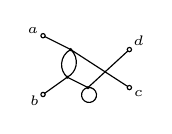
\begin{tikzpicture}[x=0.340cm, y=0.340cm, line width=0.420pt, baseline={([yshift=-0.6ex]0,0)}]
  \draw (-1.098,1.098) -- (-0.065,0.581);
  \draw (-1.098,-1.098) -- (-0.194,-0.452);
  \draw (2.127,-0.839) -- (-0.065,0.581);
  \draw (2.127,0.581) -- (0.581,-0.839);
  \draw (-0.065,0.581) arc[start angle=117.299, end angle=228.451, radius=0.631];
  \draw (-0.065,0.581) arc[start angle=48.451, end angle=-62.701, radius=0.631];
  \draw (-0.194,-0.452) -- (0.581,-0.839);
  \draw (0.581,-0.839) arc[start angle=98.011, end angle=458.011, radius=0.280];
  \fill (-0.065,0.581) circle (0.064);
  \fill (-0.194,-0.452) circle (0.064);
  \fill (0.581,-0.839) circle (0.064);
  \draw[fill=white] (-1.098,1.098) circle (0.080);
  \draw[fill=white] (-1.098,-1.098) circle (0.080);
  \draw[fill=white] (2.127,-0.839) circle (0.080);
  \draw[fill=white] (2.127,0.581) circle (0.080);
  \node[font=\tiny, inner sep=0pt, anchor=333] at (-1.250,1.174) {$a$};
  \node[font=\tiny, inner sep=0pt, anchor=36] at (-1.236,-1.197) {$b$};
  \node[font=\tiny, inner sep=0pt, anchor=147] at (2.270,-0.932) {$c$};
  \node[font=\tiny, inner sep=0pt, anchor=223] at (2.252,0.696) {$d$};
\end{tikzpicture}}
\diagramgap
\mbox{$\displaystyle +\,\frac{1}{4}$\,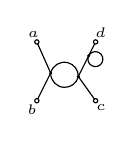
\begin{tikzpicture}[x=0.340cm, y=0.340cm, line width=0.420pt, baseline={([yshift=-0.6ex]0,0)}]
  \draw (-1.098,1.098) -- (-0.581,-0.065);
  \draw (-1.098,-1.098) -- (-0.581,-0.065);
  \draw (1.098,-1.098) -- (0.452,-0.194);
  \draw (1.098,1.098) -- (0.839,0.581);
  \draw (-0.581,-0.065) arc[start angle=178.901, end angle=346.849, radius=0.524];
  \draw (-0.581,-0.065) arc[start angle=166.849, end angle=-1.099, radius=0.524];
  \draw (0.452,-0.194) -- (0.839,0.581);
  \draw (0.839,0.581) arc[start angle=153.435, end angle=513.435, radius=0.280];
  \fill (-0.581,-0.065) circle (0.064);
  \fill (0.452,-0.194) circle (0.064);
  \fill (0.839,0.581) circle (0.064);
  \draw[fill=white] (-1.098,1.098) circle (0.080);
  \draw[fill=white] (-1.098,-1.098) circle (0.080);
  \draw[fill=white] (1.098,-1.098) circle (0.080);
  \draw[fill=white] (1.098,1.098) circle (0.080);
  \node[font=\tiny, inner sep=0pt, anchor=294] at (-1.167,1.253) {$a$};
  \node[font=\tiny, inner sep=0pt, anchor=63] at (-1.174,-1.250) {$b$};
  \node[font=\tiny, inner sep=0pt, anchor=126] at (1.197,-1.236) {$c$};
  \node[font=\tiny, inner sep=0pt, anchor=243] at (1.174,1.250) {$d$};
\end{tikzpicture}}
